\documentclass[a4paper]{article}
\usepackage{cmap}
\usepackage{mathtext}
\usepackage{amssymb}
\usepackage{amsmath}
\usepackage[russian]{babel}
\usepackage{indentfirst}
\usepackage[pdftex]{graphicx}
\usepackage{multirow}
\usepackage{mathrsfs}
\usepackage{siunitx}
\usepackage[left=2cm,right=2cm,top=2cm,bottom=2cm]{geometry}
\usepackage{fancyhdr}
\pagestyle{fancy}
\newcommand{\rref}[1]{(\ref{#1})}
\newcommand{\mbf}{\mathbf}
\newcommand{\picref}[1]{рис. \ref{#1}}
\newcommand{\Equip}[3]{
	
	{\bf #1:} $\Delta = \pm #2$ \si{#3}}
\newcommand{\equip}[1]{
	
	{\bf #1}}
\newcommand{\labname}{Релаксационные колебания.} 	% название пиши здесь
\newcommand{\labnum}{3.2.8.}										% номер вводи здесь
\fancyfoot{}
\fancyhead[RE, RO]{\thepage}
\fancyhead[LE, LO]{Лабораторная работа \labnum \space \labname}
\title{Лабораторная работа \labnum \space \labname} % Название работы здесь
\author{Иван Сладков}
\begin{document}
\maketitle
\thispagestyle{empty}
\section{Аннотация}
В данной работе проводится изучение вольт-амперной характеристики нормального тлеющего разряда; исследуются свойства релаксационного генератора на стабилитроне.

\section{Теоретические сведения}

Колебательные системы, как правило, имеют два накопителя, между которыми происходит перекачка энергии. Встречаются, однако, колебательные системы, содержащие всего один накопитель энергии. Одним из примером таких схем является схема на рис. \ref{fig:scheme}. Разряду конденсатора можно придать периодический характер, возобновляя зарядку через постоянные промежутки времени. В данной работе для этого применяется газоразрядный диод.


ВАХ такого диода (рис. \ref{fig:VAH}) не подчиняется закону Ома. При малых напряжениях лампа не пропускает ток. Он возникает, если разность потенциалов на её электродах достигает напряжения зажигания $ V_1 $. Дальнейшее возрастание тока с увеличением напряжения практически линейно. При уменьшении напряжения на диоде, лампа гаснет при напряжении гашения $ V_2 < V_1 $. 

\begin{figure}[tbp]
	\centering
	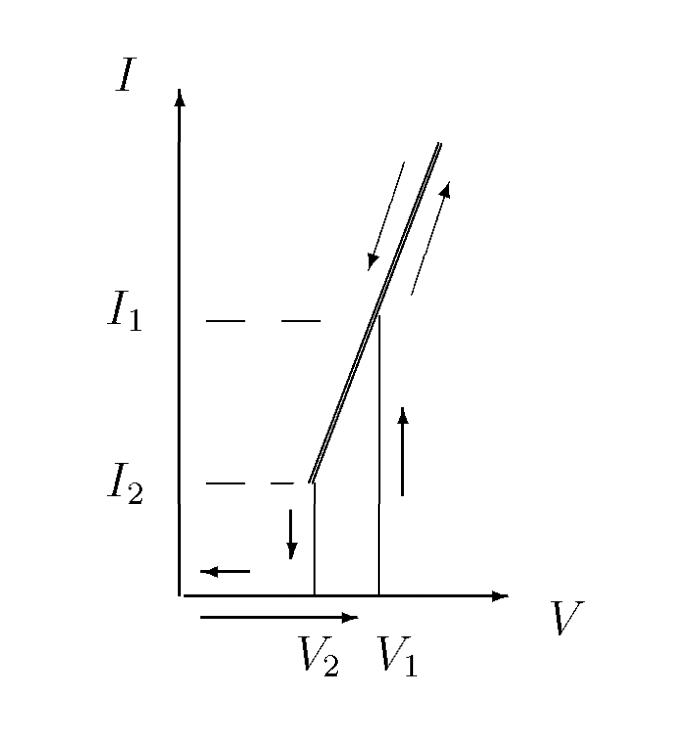
\includegraphics[width=0.8\linewidth]{VAH}
	\caption{ВАХ газонаполненного диода}
	\label{fig:VAH}
\end{figure}

\begin{figure}[tpb]
	\centering
	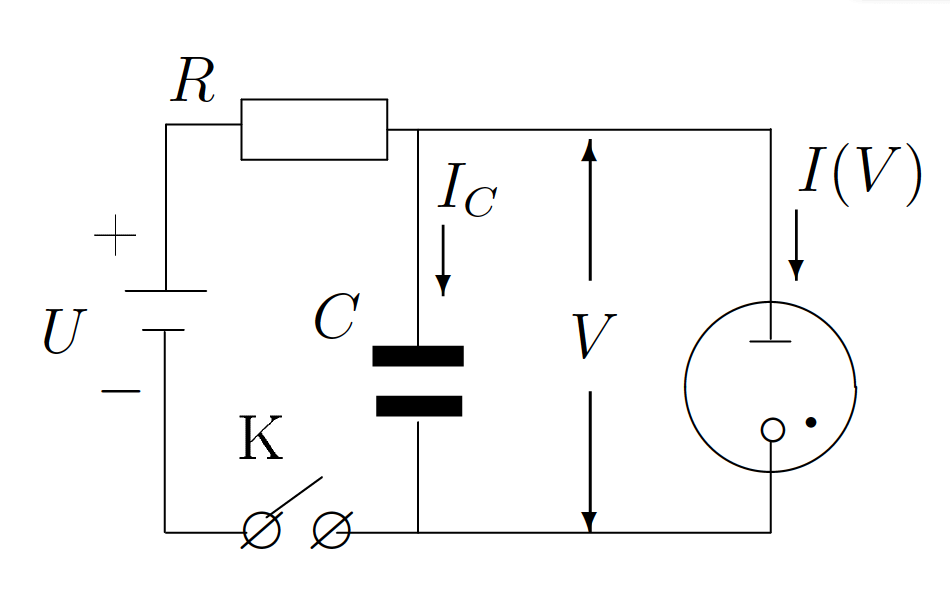
\includegraphics[width=0.8\linewidth]{Scheme}
	\caption{Схема, реализующая релаксационные колебания}
	\label{fig:scheme}
\end{figure}

Релаксационные колебания возникают, если сопротивление $ R $ достаточно велико. Тогда в момент замыкания ключа конденсатор начнёт заряжаться, и при $ V\ge V_1 $ загорится лампа. Тогда конденсатор начнёт разряжаться через неё и $ V $ станет меньше $ V_2 $. Лампа погаснет. Конденсатор вновь начнёт заряжаться.

При стационарном режиме ($I, U = \mathrm{const} $),
\begin{equation}\label{k}
	I_{ст} = \frac{U-V}{R},	
\end{equation}
тогда $ R_{кр} $ -- минимальное сопротивление, при котором возникают колебания:
\begin{equation}\label{ркр}
	R_{кр} = \frac{U-V_2}{I_2}.
\end{equation}

Найдём период. При погасшей лампе,
\begin{equation*}\label{key}
	R C \frac{d V}{d t} = U - V,
\end{equation*}
отсюда
\begin{equation*}\label{key}
	V = U - (V - V_2)\exp \frac{-t}{R C}.
\end{equation*}
В момент зажигания $ V = V_1 = V(\tau_З) $,
\begin{equation*}\label{key}
	V_1 = U - (V_1 - V_2)\exp \frac{-\tau_З}{R C}.
\end{equation*}
Тогда для периода:
\begin{equation}\label{y}
	T \approx \tau_З = R C \ln \frac{U-V_2}{U-V_1}.
\end{equation}
Здесь считаем, что 
\begin{equation}\label{усл}
	 \tau_Р \ll \tau_З,
\end{equation}
где $ \tau_Р $ -- время разрядки. Также необходимо пренебречь паразитными ёмкостями, индуктивностями, и считать, что период колебаний существенно больше времени развития разряда.


\section{Оборудование и инструментальные погрешности}

В работе используются 2 схемы: 1-я для снятия ВАХ (\picref{fig:s1}), 2-я для исследования релаксационного генератора (\picref{fig:s2}).

\begin{figure}[tbp]
	\centering
	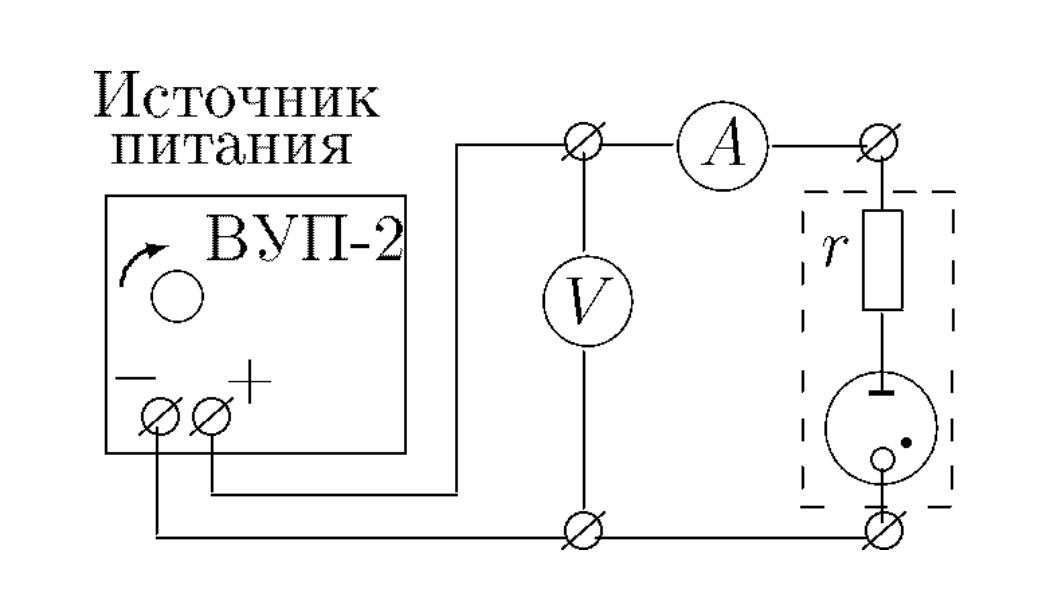
\includegraphics[width=0.8\linewidth]{Scheme1}
	\caption{Схема для исследования ВАХ}
	\label{fig:s1}
\end{figure}

\begin{figure}[tbp]
	\centering
	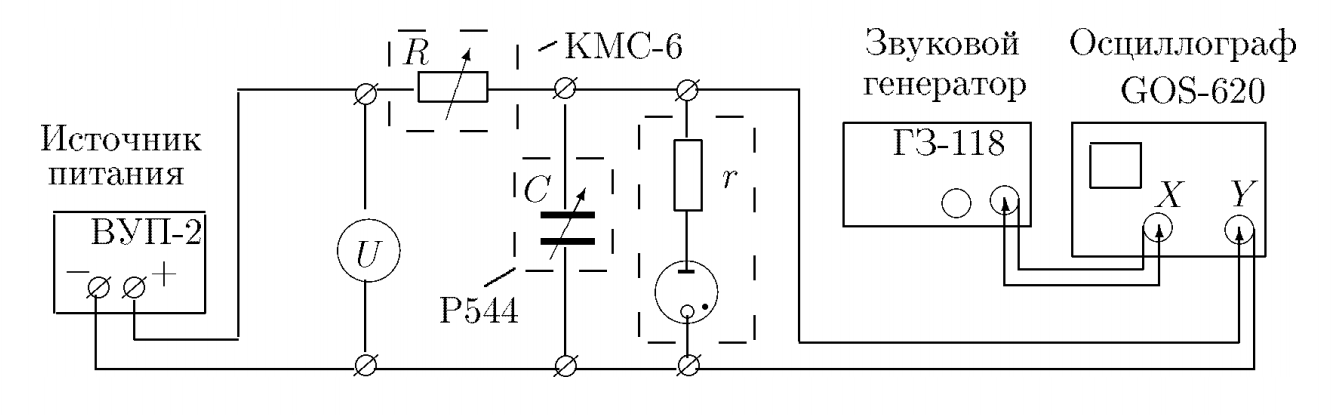
\includegraphics[width=0.8\linewidth]{Scheme2}
	\caption{Схема для исследования релаксационного генератора}
	\label{fig:s2}
\end{figure}

\Equip{Амперметр}{10}{\micro \ampere}
\Equip{Вольтметр}{10}{\milli \volt}
\equip{Стабилитрон СГ-2 (газонаполненный диод) на монтажной панели}: $ r = \SI{5.2}{\kilo \ohm} $
\equip{Магазин сопротивлений}
\equip{Магазин ёмкостей}
\equip{Источник питания}
\equip{Осциллограф}
\equip{Генератор частоты}

\section{Результаты измерений}
\emph{Все измерения и расчёты в СИ.}

\subsection{ВАХ стабилитрона}

Вольт-амперная характеристика стабилитрона в таблице \ref{tab:VAH}.
\begin{table}[h]
	\centering
	\begin{tabular}{|l|l||l|l|}
		\hline
		$U_{возр}\pm 0.01\; В$ & $I_{возр}\pm 0.01\; мА$ & $U_{уб}\pm 0.01\; В$ & $I_{уб}\pm 0.01\; мА$ \\ \hline
		5.87   & 0.01 & 110.8  & 6.9  \\ \hline
		13.96  & 0.01 & 100.79 & 5.13 \\ \hline
		48.61  & 0.01 & 95.3   & 4.17 \\ \hline
		69.11  & 0.01 & 90.2   & 3.2  \\ \hline
		90.5   & 0.01 & 85.7   & 2.4  \\ \hline
		93.59  & 3.81 & 80.8   & 1.46 \\ \hline
		99.9   & 4.97 & 77.9   & 0.01 \\ \hline
		109.9  & 6.86 & 60.3   & 0.01 \\ \hline
		120.88 & 8.78 & 41.54  & 0.01 \\ \hline
		124.4  & 9.44 & 22.15  & 0.01 \\ \hline
	\end{tabular}
	\caption{Снятие ВАХ}
	\label{tab:VAH}
\end{table}

При поиске критических значений $ V, I $ получена таблица \ref{tab:зажигание}.
\begin{table}[h]
	\centering
	\begin{tabular}{|l|l|l|l|}
		\hline
		$V_1 \pm 0.01 \;В$ & $I_1 \pm 0.01 \;мА$ & $V_2 \pm 0.01 \;В$ & $I_2 \pm 0.01 \;мА$ \\ \hline
		90.31              & 3.26                & 81.4               & 1.35                \\ \hline
		91.7               & 3.50                & 79.0               & 1.20                \\ \hline
		90.3               & 3.27                & 80.0               & 1.30                \\ \hline
	\end{tabular}
	\caption{К определению напряжений зажигания и гашения }
	\label{tab:зажигание}
\end{table}

По осциллограмме пилообразного напряжения на диоде при $ U = 110 $ В найдём:
\begin{equation*}\label{key}
	\tau_З \approx 46\; мс,
\end{equation*}
\begin{equation*}\label{key}
	\tau_Р \approx 1.5 мс.
\end{equation*}
При этом выполнено $ \tau_Р\ll \tau_З $.

\subsection{Релаксационный генератор}
В дальнейших измерениях $ U = 130.7\; В $, т. к. иначе происходящие в системе процессы становятся малозаметными.
Уменьшая сопротивление, найдём:
\begin{equation*}\label{key}
	R_{кр} = 210 \pm 1 \; кОм.
\end{equation*}
Для сравнения, по формуле \eqref{ркр}, 
\begin{equation*}\label{key}
	R_{кр} \approx \frac{130-80}{1.20} = 38.4 \pm 0.5 \; кОм.
\end{equation*}
Теоретическое и экспериментальное значения $ R_{кр} $ существенно отличаются. Это может быть связано  с тем, что не учтены процессы деионизации и установления разряда или с тем, что формула \eqref{k} задана для стационарного режима и не учитывает регулярную зарядку/разрядку конденсатора.

\subsection{Фигуры Лиссажу и частота колебаний}

Фигуры Лиссажу 1:1, 2:1, 3:1 изображены на рис. \ref{fig:11}, \ref{fig:12}, \ref{fig:31} соответственно. Для соотношений 1:2, 1:3 фигуры получить не удалось. 
\begin{figure}[tbp]
	\centering
	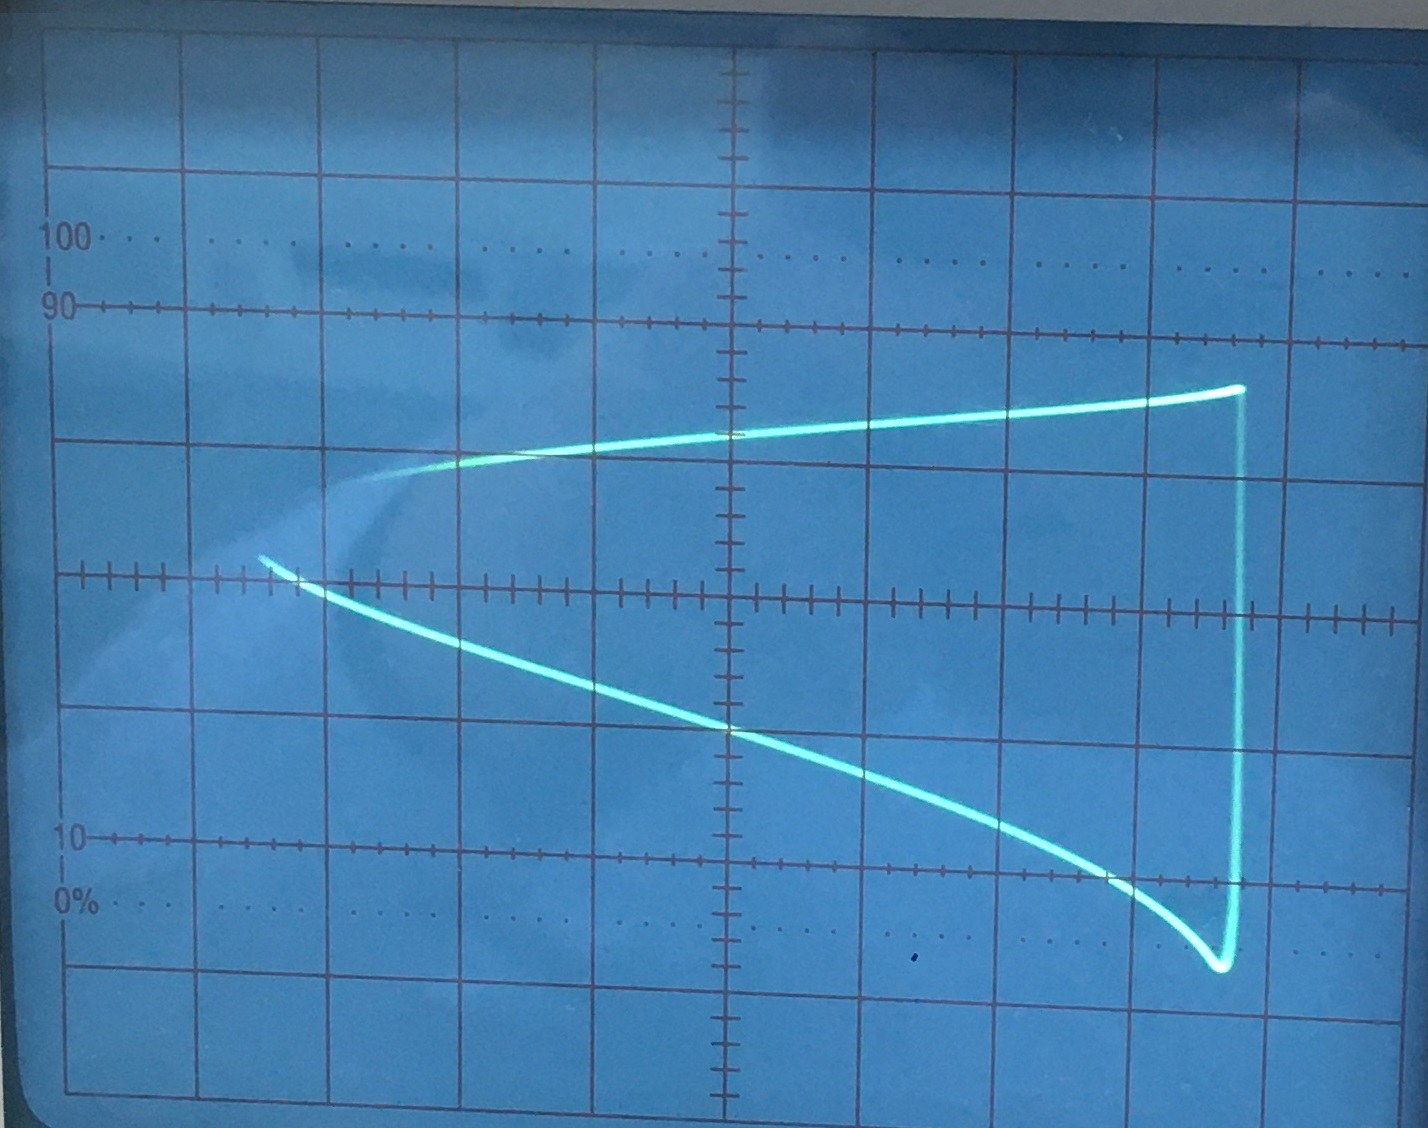
\includegraphics[width=0.5\linewidth]{Осциллограмма}
	\caption{Лиссажу 1:1}
	\label{fig:11}
\end{figure}
\begin{figure}[tbp]
	\centering
	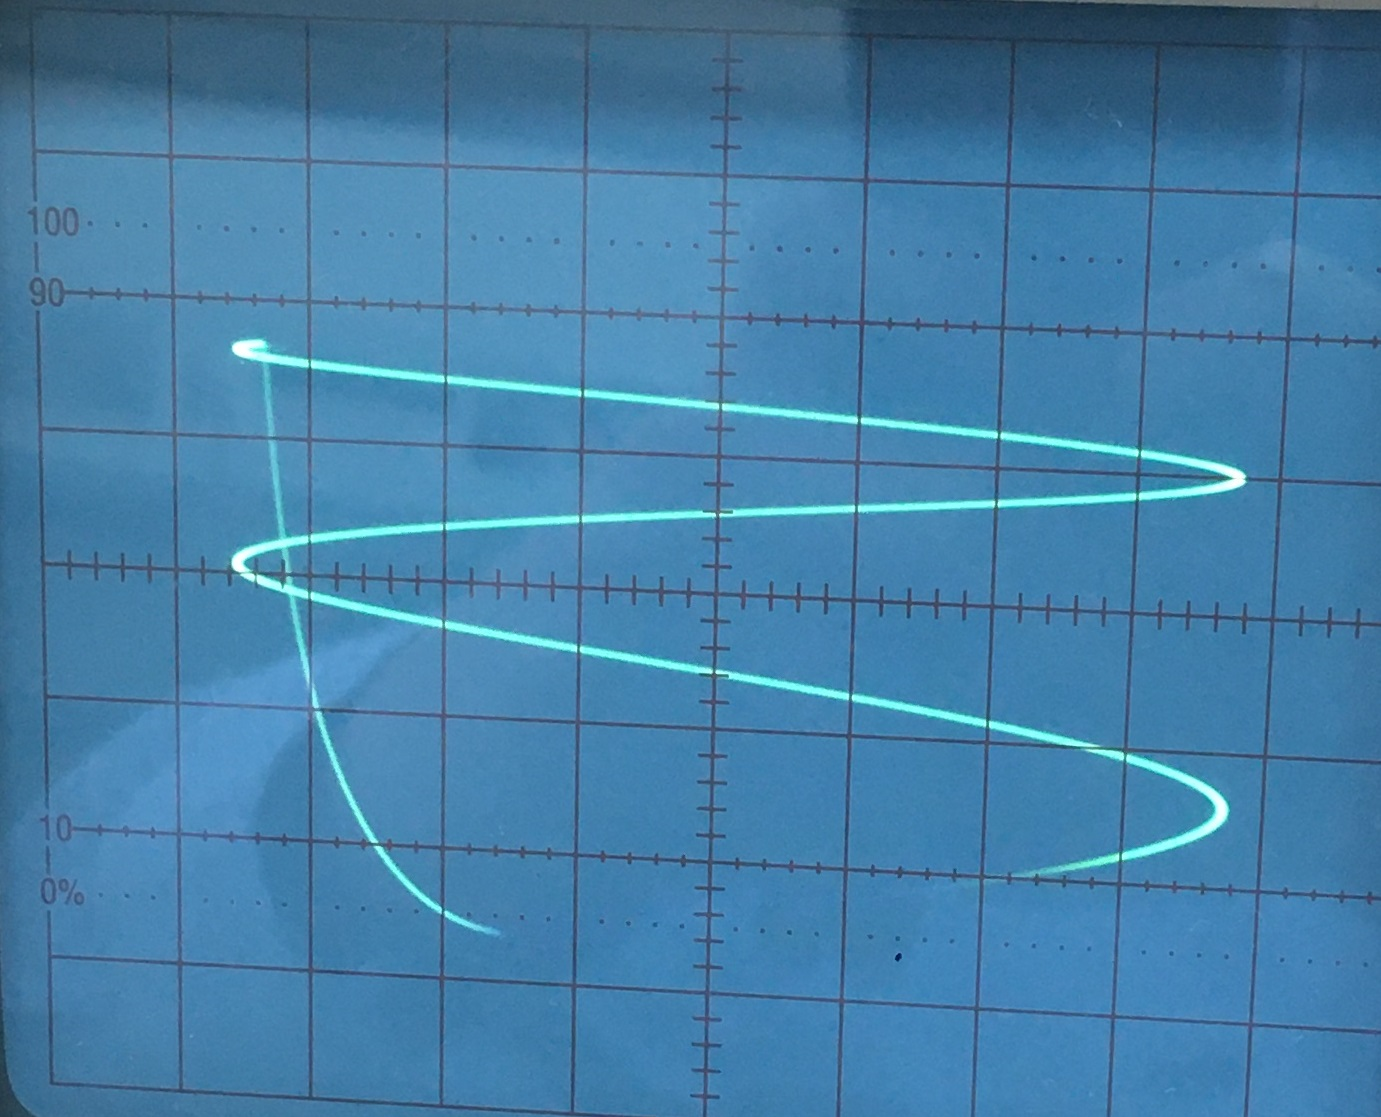
\includegraphics[width=0.5\linewidth]{21}
	\caption{Лиссажу 2:1}
	\label{fig:12}
\end{figure}
\begin{figure}[tpb]
	\centering
	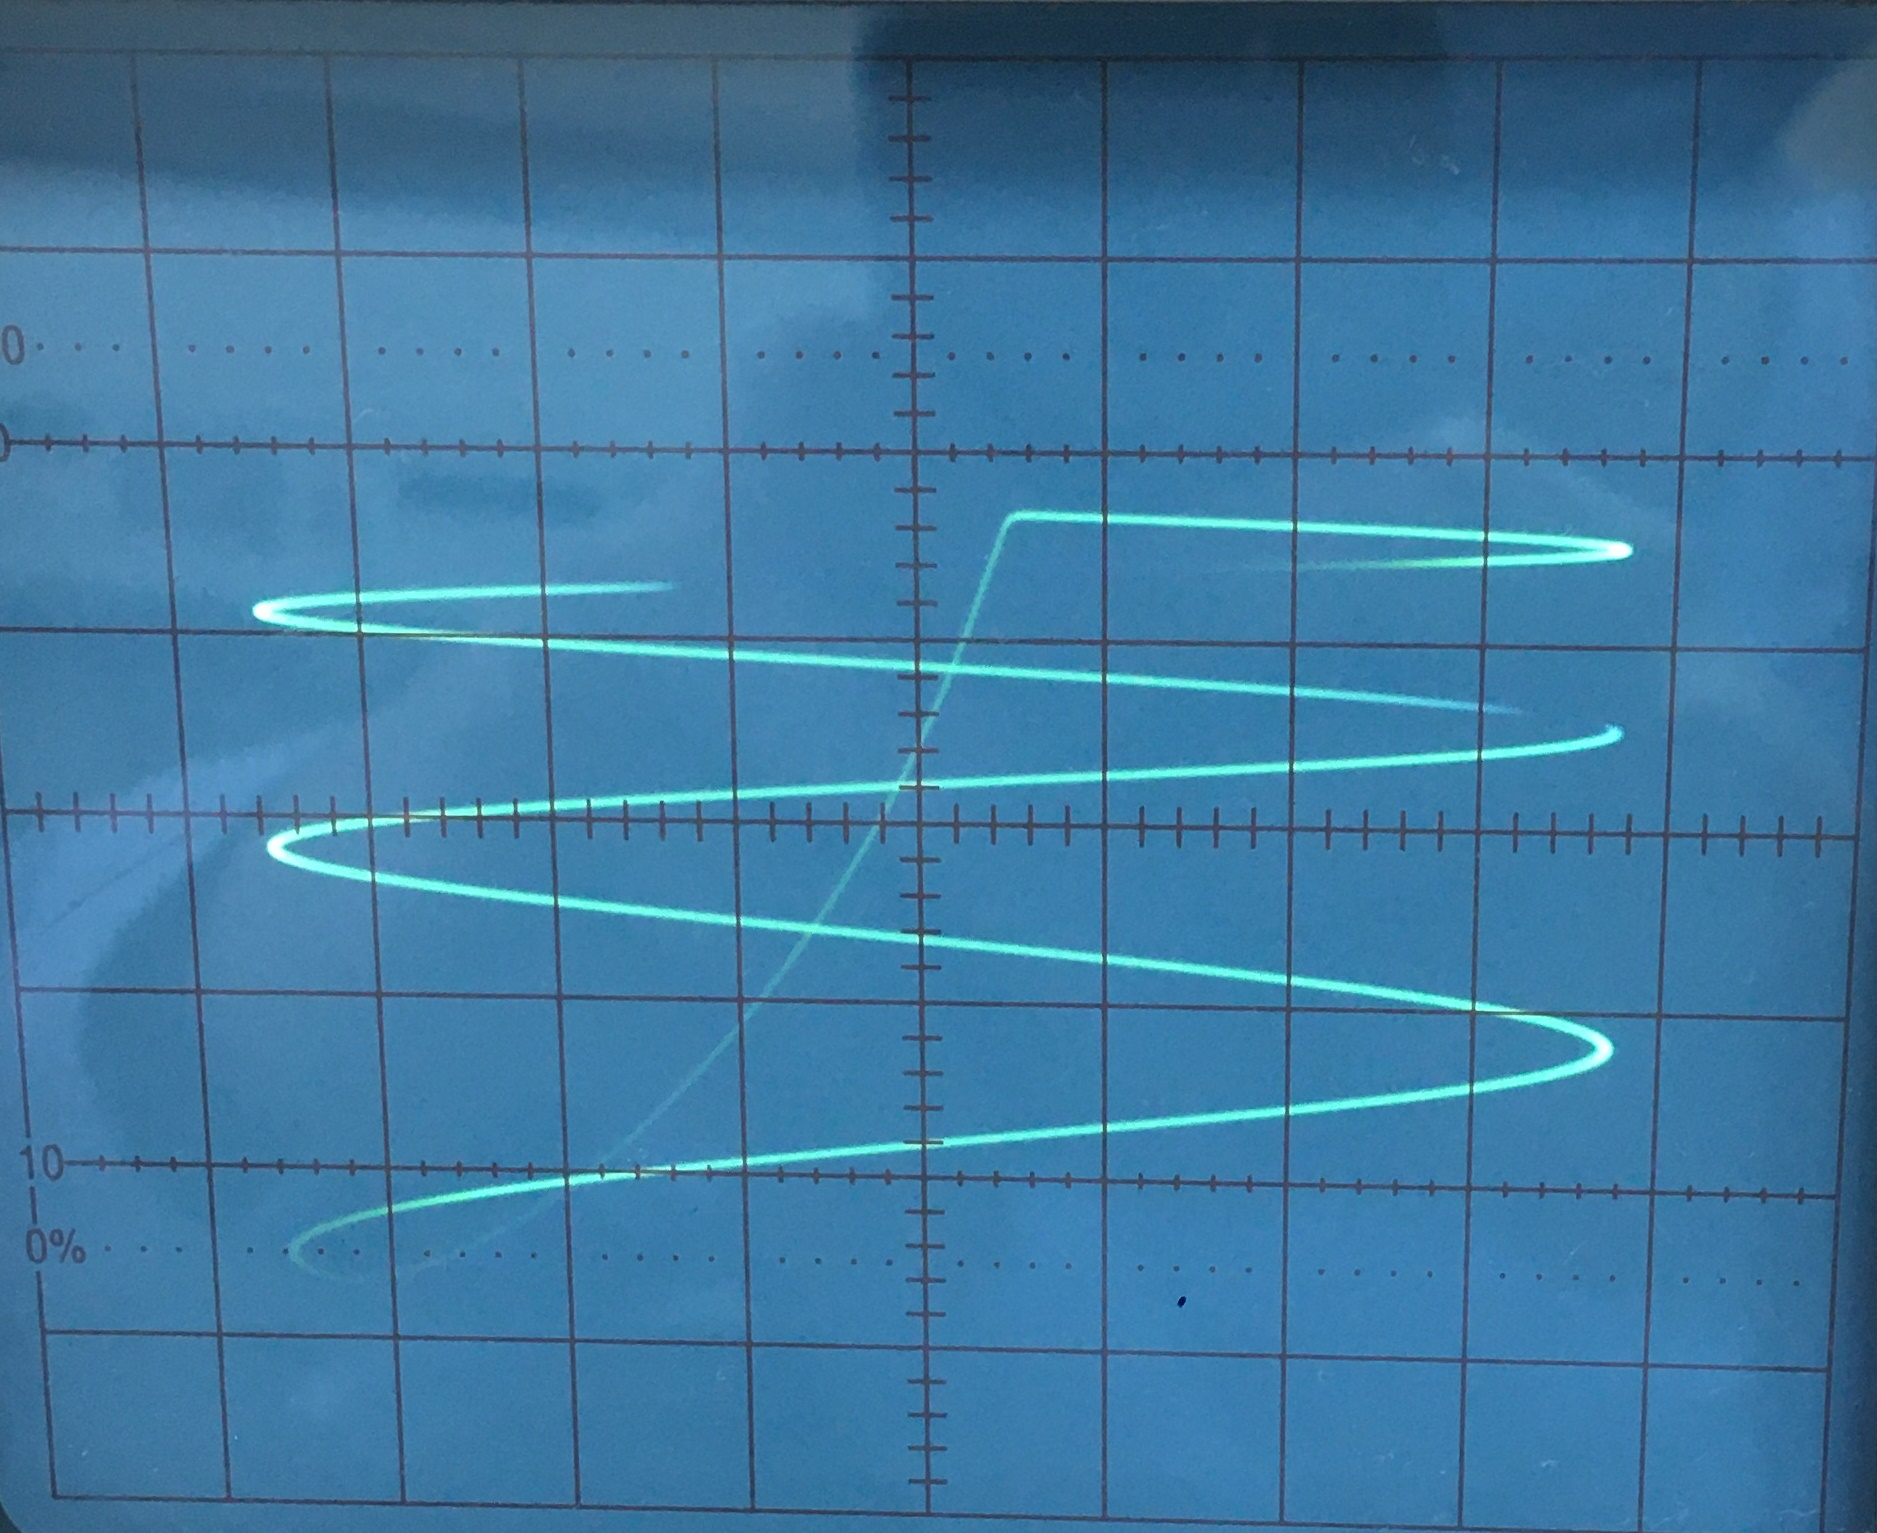
\includegraphics[width=0.5\linewidth]{31}
	\caption{Лиссажу 3:1}
	\label{fig:31}
\end{figure}

При снятии зависимости $ \nu(C) $ получены результаты табл. \ref{tab:c-nu}.
\begin{table}[h]
	\centering
	\begin{tabular}{|l|l|}
		\hline
		$C\pm 0.1\; нФ$ & $\nu \pm 1\; Гц$ \\ \hline
		50              & 52               \\ \hline
		45              & 58               \\ \hline
		40              & 67               \\ \hline
		35              & 79               \\ \hline
		30              & 96               \\ \hline
		25              & 118              \\ \hline
		20              & 162              \\ \hline
		15              & 249              \\ \hline
		10              & 431              \\ \hline
		5               & 951              \\ \hline
	\end{tabular}
	\caption{$\nu(C)$ при $R = 640\; кОм,$ $U = 130.7\; В$}
	\label{tab:c-nu}
\end{table}

При снятии зависимости $ \nu (R) $ получили результаты  в таблице \ref{tab:r-nu}.

\begin{table}[h]
	\centering
	\begin{tabular}{|l|l|}
		\hline
		$R\pm 0.001 \; кОм$ & $\nu\pm 1 \; Гц$ \\ \hline
		1000                & 33               \\ \hline
		900                 & 37               \\ \hline
		800                 & 41               \\ \hline
		700                 & 47               \\ \hline
		600                 & 55               \\ \hline
		500                 & 67               \\ \hline
		400                 & 86               \\ \hline
		300                 & 119              \\ \hline
		290                 & 126              \\ \hline
		270                 & 139              \\ \hline
		250                 & 160              \\ \hline
		230                 & 203              \\ \hline
	\end{tabular}
	\caption{$\nu (R)$ при $C = 50 нФ$, $U = 130.7 В$}
	\label{tab:r-nu}
\end{table}

\section{Обработка данных}

Построим график ВАХ стабилитрона с резистором r (\picref{fig:vahgraph}) и без него (\picref{fig:vahgraphnores}). Существование 2 различных $ I $ при одном $ U $ обусловлено падением напряжения на резисторе, которое отсутствует, когда лампа не горит.

\begin{figure}[tbp]
	\centering
	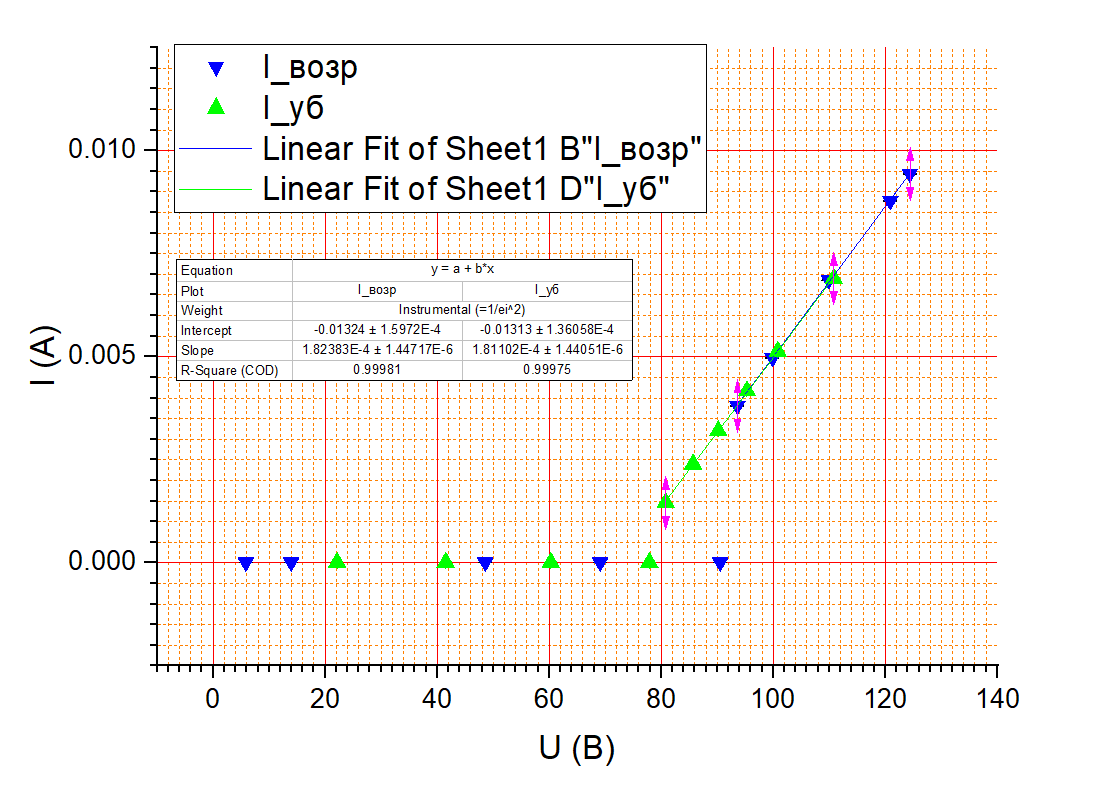
\includegraphics[width=0.8\linewidth]{vahGraph}
	\caption{ВАХ стабилитрона с резистором}
	\label{fig:vahgraph}
\end{figure}

\begin{figure}[tbp]
	\centering
	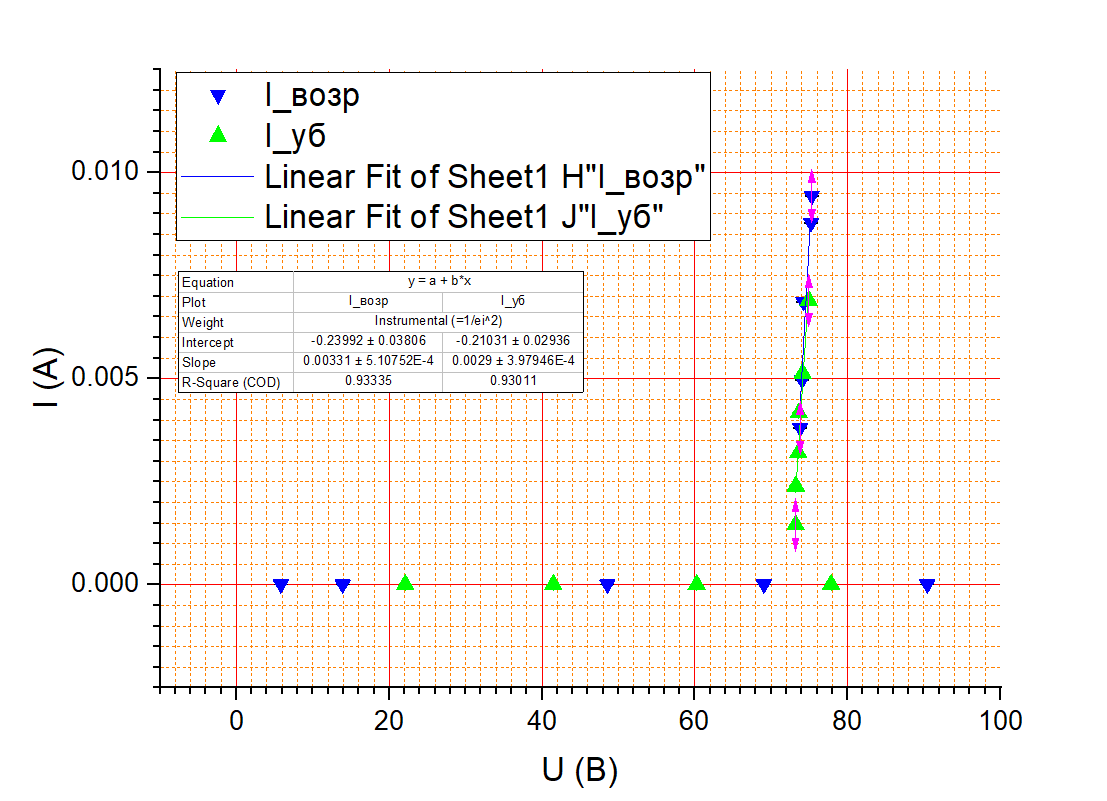
\includegraphics[width=0.8\linewidth]{vahGraphNores}
	\caption{ВАХ стабилитрона без резистора}
	\label{fig:vahgraphnores}
\end{figure}

Построим графики $ T(C), \; T(R) $ для экспериментальных и теоретических значений на \picref{a} и \picref{b}.

Наклон графиков существенно различается. Найдём динамический потенциал из \eqref{y} например для графика $ T(C) $:
\begin{equation*}\label{key}
	k = R \ln \frac{U-V_2}{U-V_1} = 420000 \pm 8000
\end{equation*}
\begin{equation*}\label{key}
	V_2 = U-(U-V_1)\exp \frac{k}{R} \approx 54 \; В
\end{equation*}

\begin{figure}[tbp]
	\centering
	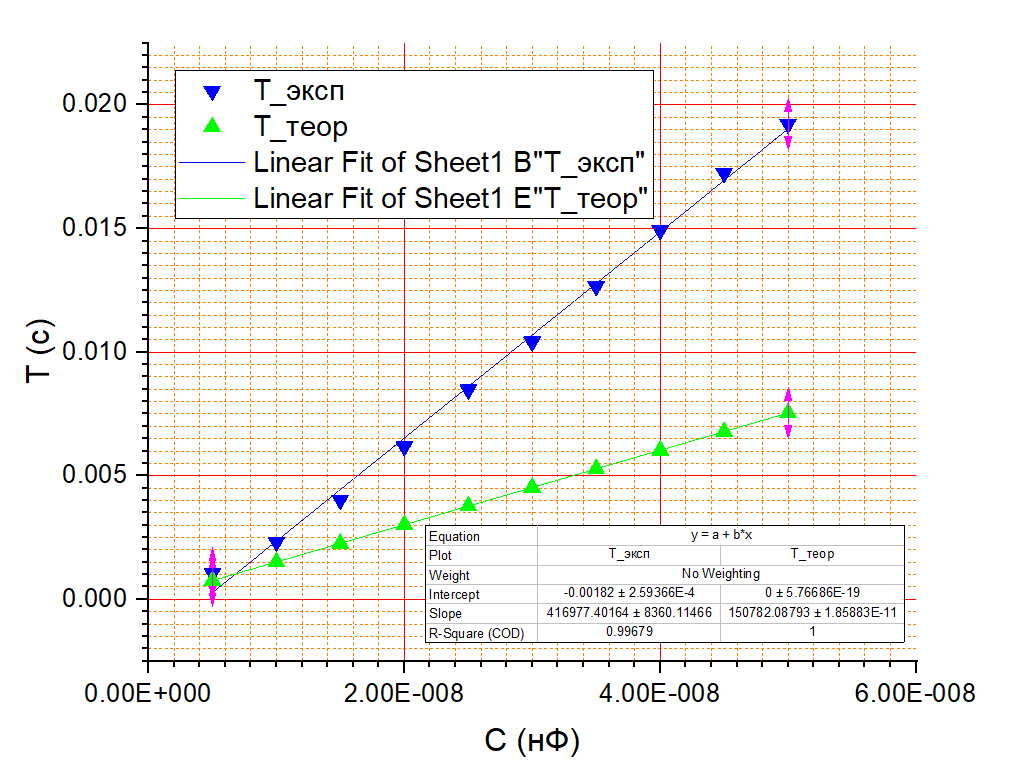
\includegraphics[width=0.8\linewidth]{T(c)}
	\caption{Зависимость $T(C)$}
	\label{a}
\end{figure}
\begin{figure}[tbp]
	\centering
	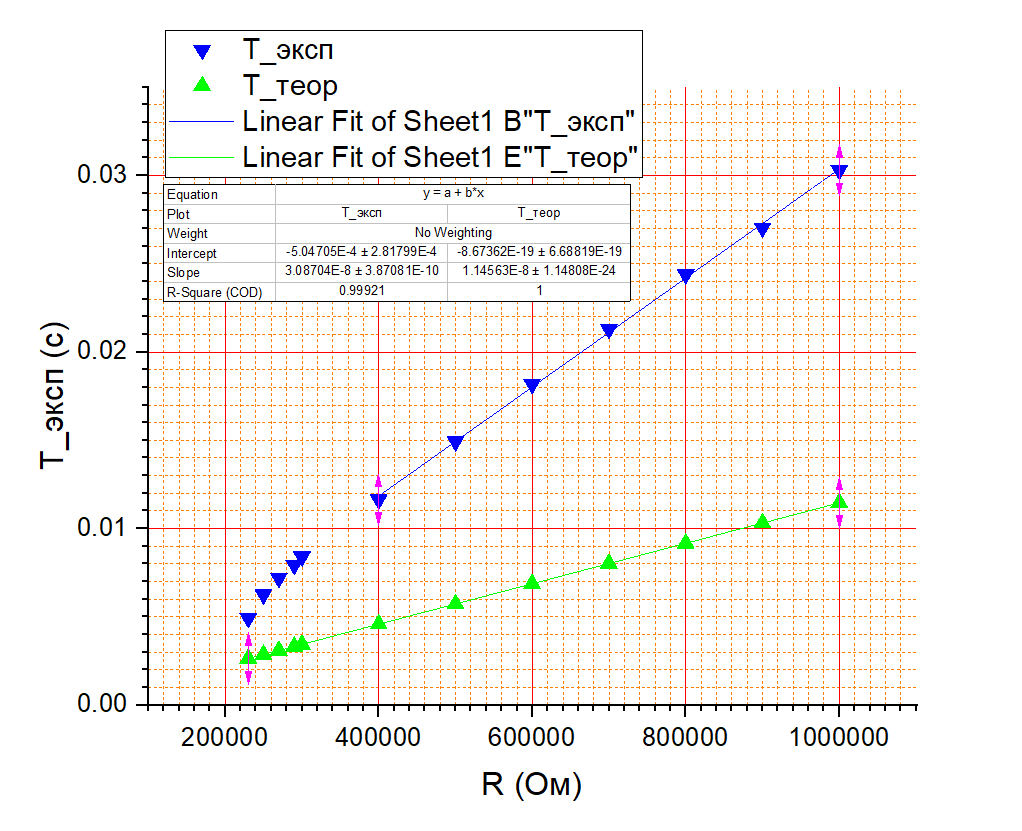
\includegraphics[width=0.8\linewidth]{T(R)}
	\caption{Зависимость $T(R)$}
	\label{b}
\end{figure}

Значит, лампа работает в динамическом режиме релаксационных колебаний (например, это может быть связано с выбором более высокого напряжения $ U $).


\section{Вывод}

Ознакомились с принципом действия газонаполненного диода в режиме стабилитрона; сняли его ВАХ. Собрали и исследовали релаксационный генератор; вычислили и нашли экспериментально его период.

\newpage
\begin{thebibliography}{9}
	\bibitem{Siv} Сивухин Д. В. \emph{Общий курс физики. Том 3 Электричество и магнетизм}, 2004
	\bibitem{kirich} Кириченко Н.А. \emph{Электричество и магнетизм.}, 2011
	\bibitem{max} \emph{Лабораторный практикум по общей физике. В 3 томах. Том 2. Электричество и магнетизм: учебное пособие} под ред. А. В. Максимычева, М. Г. Никулина
\end{thebibliography}
\end{document}